\chapter{Architettura}

In questo capitolo verranno descritte le scelte architetturali e implementative che stanno alla base del contributo di questa tesi al progetto IoE. 

Lo scenario legato alla mobilità elettrica veicolare è caratterizzato dalla presenza di diversi domini applicativi, piattaforme e parti interessate i quali necessitano di comunicare in modo unificato e trasparente. A tal fine è stato utilizzato il progetto Smart-M3 (\cite{tullio2011}) che è il cuore della nostra architettura. Appoggiandosi sulle tecnologie tipiche del \emph{Semantic Web} Smart-M3 assicura l'interoperabilità tra gli attori in gioco. 

In particolare vedremo come possono coesistere elementi reali ed elementi simulati e come il passaggio dall'uno all'altro sia assolutamente trasparente a tutti i componenti del sistema grazie all'uso di tecnologie ontology-based.

\section{Smart-M3}

Prima di parlare dei componenti strettamente legati a questo progetto è doveroso fare un introduzione alla tecnologia che fa da collante tra di essi ovvero Smart-M3. Capire come funziona Smart-M3 e quali sono i suoi principi è fondamentale al fine di comprendere a fondo il resto di questo documento.

M3 è un architettura middleware per consentire L'interoperabilità delle informazioni in maniera cross-domain, multi-vendor, multi-device, multi-piattaforma (\cite{smart2013}). Smart-M3 è la sua prima implementazione Open Source, proposta da SOFIA, un Progetto Europeo (2009-11), appartenente al framework ARTEMIS. 
La piattaforma implementa il disaccoppiamento tra produttori e consumatori di informazione. In questa architettura tutti gli attori (sensori, dispositivi, servizi, attuatori ecc..) cooperano attraverso un database RDF che è lo standard deciso dal World Wide Web Consortium per la descrizione di informazioni e concetti. L'interoperabilità è resa possibile da un modello di dati condiviso che si basa su tecnologie tipiche del Semantic Web.

Il Semantic Web è un framework sviluppato dal World Wide Web Consortium per consentire la condivisione e il riutilizzo dei dati attraverso  applicazioni, aziende e comunità eterogenee.

La figura ~\ref{fig:smart-m3} mostra il funzionamento dell'architettura M3. Il "legacy gate" è un interfaccia con il mondo esterno e di essi ne possono coesistere innumerevoli in un architettura M3.

\begin{figure}[H]
	\centering
	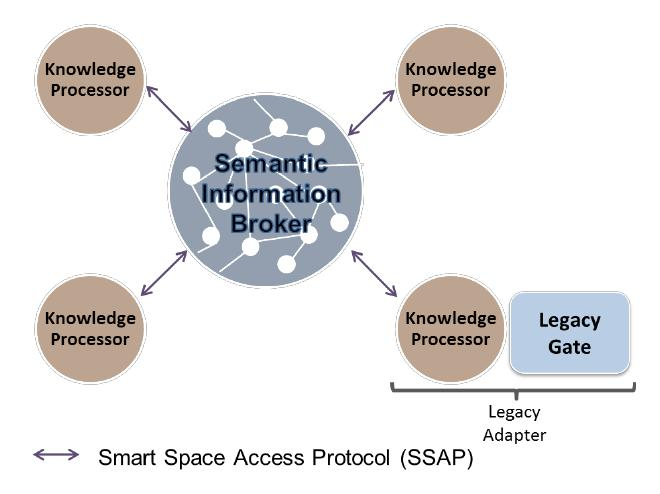
\includegraphics[width=0.5\textwidth]{assets/smart-m3.jpg}
	\caption{Architettura Smart-M3}
	\label{fig:smart-m3}
\end{figure}

\subsection{Semantic Information Broker}\label{subsec:sib}

Il \emph{Semantic Information Broker} (SIB) è l'entità responsabile della conservazione e della gestione delle informazioni condivise nell'architettura M3. Gli agenti Software che si scambiano le informazioni vengono chiamati \emph{Knowledge Processors} (KPs). L'accesso alla SIB da parte dei KP avviene attraverso lo \emph{Smart Space Access Protocol}  (SSAP), esso consiste in messaggi XML scambiati attraverso socket TCP/IP. Vengono fornite API che implementano il protocollo SSAP in diversi linguaggi.

Il SIB è un architettura a 5 livelli (\cite{smart2010}) come mostrato in figura ~\ref{fig:sib-architecture}:

\begin{enumerate}
	\item \textbf{Transport}: Questo livello consiste in una o più comunicazioni di rete a livello di trasporto che permette al SIB di comunicare con diverse reti e architetture. Il livello di trasporto è collegato a quello sottostante tramite il DBus, rendendo possibile l'aggiunta e la rimozione di connettori a runtime.
	\item \label{enum:handling}\textbf{Operation Handling}: A questo livello vengono gestite le operazioni del protocollo SSAP e ognuna di esse viene eseguita in un thread dedicato. Malgrado l'uso intensivo di thread possa degradare le performance la chiarezza di codice che ne consegue è stata ritenuta più importante.
	\item \label{enum:graph}\textbf{Graph Operations}: Questo livello gestisce le operazioni di inserimento, rimozione e query dal database RDF come richiesto dal livello ~\ref{enum:handling}. Viene eseguito all'interno di un singolo thread che schedula ed esegue le richieste provenienti dai thread che gestiscono le operazioni SSAP la quale comunicazione avviene tramite code asincrone.
	\item \textbf{Triple Operations}: A questo livello vengono gestite le operazioni SPARQL, WQL e le query basate su pattern-matching di triple RDF. Attualmente è implementato tramite Piglet, un database RDF che si appoggia ad SQL lite per la persistenza delle informazioni. Questo strato può essere tranquillamente cambiato a patto che si scriva il codice necessario ad interfacciare le operazioni a livello di grafo (~\ref{enum:graph}) con l'interfaccia fornita dal nuovo store RDF.
	\item \textbf{Persistent storage}: Quetso è il livello che assicura la persistenza dei dati.
\end{enumerate}

\subsection{I Knowledge Processor}

I Knowledge Processor (KP) sono le parti attive dell'architettura Smart-M3. Un KP interagisce con il SIB non direttamente tramite il protocollo SSAP ma tramite le Knowledge Processor Interface (KPI) ovvero delle librerie che lo implementano. Esse possono trovarsi a qualunque livello di astrazione ed essere scritte in qualunque linguaggio. Le funzioni messe a disposizione dal KPI in genere sono speculari alle operazioni del protocollo SSAP.

I KP sono quelle entità che forniscono, modificano e richiedono le informazioni le informazioni contenute nello smart-space. L'architettura dei KP è mostrata in figura ~\ref{fig:kp-architecture}.

\begin{figure}[H]
        \centering
        \begin{subfigure}[H]{0.5\textwidth}
                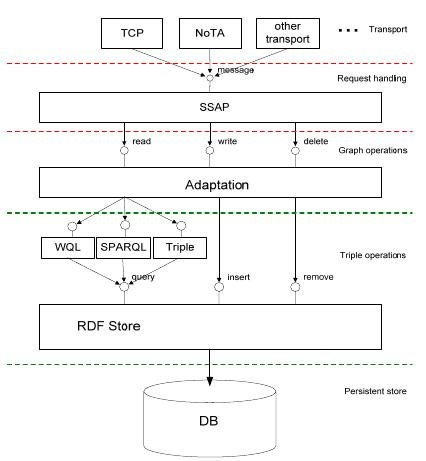
\includegraphics[width=\textwidth]{assets/sib-architecture.jpg}
                \caption{Architettura del SIB}
                \label{fig:sib-architecture}
        \end{subfigure}%
        \begin{subfigure}[H]{0.42\textwidth}
                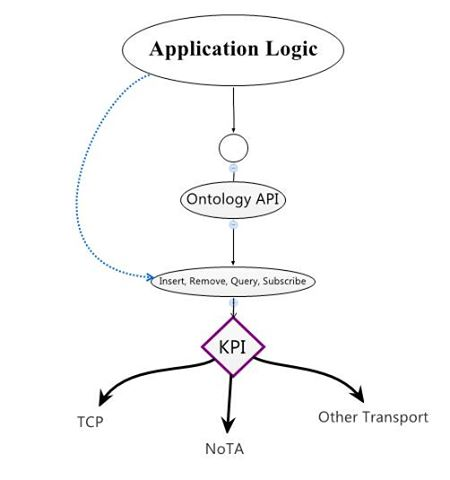
\includegraphics[width=\textwidth]{assets/kp-architecture.jpg}
                \caption{Architettura dei KP}
                \label{fig:kp-architecture}
        \end{subfigure}
        \caption{Architetture SIB e KP}
\end{figure}

\subsection{Le triple RDF}

Nell'architettura Smart-M3 le informazioni sono rappresentate in formato RDF (Resource Description Framework). In RDF le informazioni sono rappresentate come una tripletta \emph{soggetto, predicato, oggetto}. Le triple vengono memorizzate nel SIB e formano un grafo etichettato diretto il quale non necessariamente è un grafo connesso.

\subsection{Ontologie}

Mentre RDF fornisce il modello di dati standard per la rappresentazione delle informazioni, l'uso di un linguaggio ontologico è indispensabile per assegnare una semantica all'informazione. Linguaggi ontologici come RDFS e OWL forniscono un vocabolario comune. L'uso di una ontologia comune consente a tutti gli attori (uomini e macchine) di capire reciprocamente la semantica delle informazioni e di cooperare in simbiosi attraverso il SIB. Smart-M3 è agnostico rispetto all'ontologia e quindi consente agli sviluppatori di scegliere il modo migliore di modellare le informazioni al fine di soddisfare le esigenze funzionali del dominio applicativo indirizzato.

\subsection{Sottoscrizioni}

Un aspetto fondamentale di questa tecnologia è il meccanismo delle sottoscrizioni grazie al quale è possibile ricevere notifiche al variare di set di triple. Le sottoscrizioni sono determinanti nella nostra architettura perché, come vedremo più avanti (Sez. ~\ref{sec:protocol}), sono alla base dei protocolli di scambio dati tra i componenti del sistema.

\subsection{SPARQL}

SPARQL, si pronuncia sparkle, (acronimo ricorsivo di SPARQL Protocol and RDF Query Language) è il linguaggio standard de facto per interrogare dei dataset RDF. Come si può dedurre dal nome stesso SPARQL non è semplicemente un linguaggio di interrogazione di dati RDF, ma definisce anche il protocollo applicativo utilizzato per comunicare con le sorgenti RDF (si tratta di un binding su HTTP).

Così come SQL riflette, nella rappresentazione della query, il modello relazionale sottostante, allo stesso modo SPARQL basa la rappresentazione della query sul concetto di tripla e di grafo. Il meccanismo alla base della rappresentazione di una query e della ricerca della sua risposta è il graph matching. La query rappresenta un pattern di un grafo (RDF) e la risposta alla query sono tutte le triple (sotto-grafo) che fanno match con il pattern.

\subsection{Il protocollo SSAP}

L'SSAP (\emph{Smart Space Access Protocol}) è il protocollo con cui si comunica con il SIB. Il protocollo è session-based, i KP che vogliono comunicare con lo smart-space dovranno prima aderirvi con un operazione di Join prevista dall'SSAP. Il KP fornisce le sue credenziali nel messaggio di Join, il SIB esamina le credenziali e decide se accetare il KP o meno. Dopo l'operazione di Join, il KP può eseguire le altre operazioni. 
L'SSAP è il punto di integrazione principale dell'architettura Smart-M3. Le implementazioni di SIB e KP devono implementare tutte le operazioni del protocollo SSAP al fine di garantire l'interoperabilità.

Le operazioni supportate dal protocollo SSAP sono:

\begin{itemize}
	\item \textbf{JOIN}: Associa il KP allo smart-space solo se le credenziali verranno ritenute valide. Determina l'inizio della sessione.
	\item \textbf{LEAVE}: Determina il termine dell'associazione con lo smart-space e quindi la fine della sessione. Da questo momento in poi non potranno essere eseguite altre operazione di associazione allo smart-space.
	\item \textbf{INSERT}: Operazione atomica di inserzione di un Grafo, formato da triple RDF, nel SIB.
	\item \textbf{REMOVE}: Operazione atomica di rimozione di un Grafo, formato da triple RDF, nel SIB.
	\item \textbf{UPDATE}: Operazione atomica di aggiornamento di un Grafo, formato da triple RDF, nel SIB. In realtà si tratta di una combinazione di DELETE e INSERT eseguita in modo atomico dove l'operazione di DELETE viene eseguita per prima.\textsl{•}
	\item \textbf{QUERY}: Richiesta di informazioni contenute nel SIB attraverso una delle modalità supportate.
	\item \textbf{SUBSCRIBE}: Sottoscrizione a un set di triple contenute nel SIB. Il KP riceve una notifica quando avviene un cambiamento su una di queste triple.
	\item \textbf{UNSUBSCRIBE}: Cancella una sottoscrizione.
\end{itemize}

%\begin{figure}
%	\centering
%	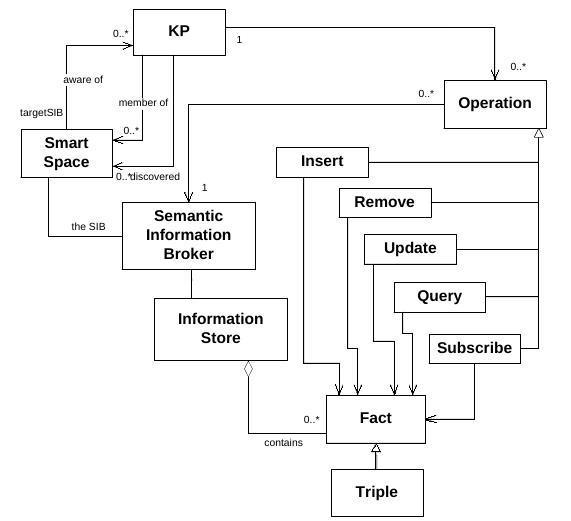
\includegraphics[width=0.5\textwidth]{assets/smart-m3-domain.jpg}
%	\caption{Smart-M3 modello di dominio}
%	\label{fig:smart-m3-domain}
%\end{figure}

\section{Il Modello Ontologico}

In questa sezione verrà spiegato come sono stati modellati i dati attraverso un ontologia. Il modello ontologico è stato ereditato dalla progetto di Tesi di \emph{Federico Montori} (\cite{montori2012}). Io ho contribuito espandendolo al fine di adattarlo ai nuovi requisiti funzionali sorti durante lo sviluppo del progetto. Verranno quindi mostrate gli aspetti dell'ontologia necessari a comprendere il resto della trattazione e verranno approfondite le modifiche da me apportate.

\subsection{Introduzione}

L'ontologia è definibile come una rappresentazione formale ed esplicita di una concettualizzazione condivisa di un dominio di interesse.

L'ontologia presenta le seguenti proprietà:

\begin{itemize}
	\item \textbf{Rappresentazione Formale}: Utilizza pertanto un linguaggio logico processabile da elaboratori.
	\item \textbf{Esplicita}: Cioè non ambigua e tale da chiarire ogni assunzione fatta.
	\item \textbf{Concettuale}: È una concettualizzazione cioè una vista astratta e semplificata del dominio di interesse
	\item \textbf{Condivisa}: Determinata dal consenso di una pluralità il più ampia possibile di soggetti.
\end{itemize}

Lo scopo delle ontologie è quindi descrivere delle basi di conoscenze, effettuare delle deduzioni su di esse e integrarle tra le varie applicazioni. Per descrivere le ontologie viene utilizzato il linguaggio OWL (\emph{Ontology Web Language}) che è un estensione di RDF. È un linguaggio di markup per rappresentare esplicitamente significato e semantica di termini con vocabolari e relazioni tra gli stessi.

I linguaggi della famiglia OWL sono in grado di creare \emph{classe}, \emph{proprietà}, \emph{istanze} e le relative \emph{operazioni}.


\subsection{Classi di IoE}

Una classe è una collezione di oggetti che corrisponde alla descrizione logica di un concetto. Da una classe si possono creare un numero arbitrario di istanze mentre ad un istanza può corrispondere ad una, nessuna o molteplici classi.\newline
Una classe può essere sottoclasse di un'altra classe, ereditando le caratteristiche della super-classe. Tutte le classi sono sottoclasse di \code{owl:Thing}.

Nel modello di dati utilizzato in questo progetto si è cercato di tenere disaccoppiato il concetto di dato dalle altre entità fisiche. Ne consegue che tutte le entità fisiche sono sottoclassi dirette di \code{owl:Thing}, mentre le classi destinate a rappresentare i dati sono sottoclasse di \code{ioe:Data} che a sua volta è sottoclasse di \code{owl:Thing}.\newline
Nel resto di questo documento userò il prefisso \code{ioe:} come abbreviazione di \emph{http://www.m3.com/2012/05/m3/ioe-ontology.owl\#} che è il namespace scelto per l'ontologia. In generale userò questo prefisso per distinguere le classi dell'ontologia dalle classi Java che come vedremo nella sezione ~\ref{subsec:ioe-lib} hanno lo stesso nome essendo mapping diretto di quest'ultime.

\subsection{Sottoclassi di owl:Thing}\label{subsec:thing}

Come già accennato tutte le entità fisiche del nostro modello ontologico sono sottoclasse diretta di owl:Thing. Quellla mostrata di seguito è una lista delle Classi utilizzate in questo progetto, vengono omesse quelle che sono attualmente irrilevanti o inutilizzate.

\begin{description}
	\item \textbf{Person}: Questa classe rappresenta il concetto di persona. Ad ogni persona possono essere associati diversi veicoli (Vehicle), diverse richieste di ricarica (Reservation), nonché una storia delle ricariche effettuate (Recharge). Il concetto di persona viene utilizzato ai fini di autenticazione e in un futuro potrà essere determinante ai fini della fatturazione che il provider energetico eseguirà in seguito alle ricariche.
	\item \textbf{Vehicle}: Rappresenta il concetto di Veicolo Elettrico, siccome i veicoli non elettrici sono irrilevanti al fine di questa trattazione è stata usata direttamente questa classe allo scopo. Ad ogni veicolo sono ovviamente associati i dati della batteria (BatteryData) che verranno trattati nella sezione relativa alle sottoclassi di \code{ioe:Data} (~\ref{subsec:ioe-data});
	\item \textbf{GridConnectionPoint}: Il \emph{Grid Connection Pointer} (GCP) è la stazione di ricarica. Esso contiene almeno un EVSE che invece rappresenta la colonnina dove ci si ricarica effettivamente. Il rapporto tra un GCP e gli EVSE è lo stesso che intercorre tra una stazione di rifornimento e le pompe di benzina. 
	\item \textbf{EVSE}: Il \emph{Electrical Vehicle Supply Equipment} è il punto in cui il veicolo si connette alla rete elettrica. Una volta connesso può sia ricaricare la sua batteria che cedere energia alla smart-grid. Un EVSE ha diversi connettori (Connector) per adattarsi ai vari tipi di presa posseduti dai veicoli elettrici. Inoltre, ogni EVSE, ha una lista di prenotazioni associate.
	\item \textbf{ChargeProfile}: È l'insieme dei parametri che caratterizzano il profilo energetico di un EVSE in un determinato istante. I parametri attualmente sono: potenza, orario di validità del profilo stesso e prezzo per unità di energia (in genere 1 kWh). Ovviamente può essere attivo un solo ChargeProfile alla volta e il variare di quest'ultimi può essere determinato da fasce orarie proprio come avviene per l'energia elettrica casalinga.
	\item \textbf{Connector}: È il connettore di ricarica ovvero il punto i contatto tra l'EVSE e l'EV. Ogni EVSE può avere diversi connettori al fine di poter essere compatibile con il maggior numero di veicoli possibile. Malgrado negli usa si stia cercando di introdurre uno standard a riguardo ormai esistono diversi tipi di connettori. 
	\item \textbf{ChargeRequest}: Richiesta di ricarica. Viene istanziata quando un utente necessita di creare una prenotazione e al suo interno sono contenuti tutti i parametri necessari a descriverla. Fa parte del protocollo di richiesta di prenotazione discusso nella sezione ~\ref{sec:protocol}. Mentre un approfondimento sulla sua struttura è trattato nella sezione ~\ref{subsubsec:chargerequest}.
	\item \textbf{ChargeResponse}: È la risposta fornita dal servizio cittadino a seguito della richiesta di prenotazione. Al suo interno contiene un riferimento alla richiesta (ChargeRequest) da cui è stata generata e una lista di opzioni di ricarica che aderiscono alla richiesta dell'utente (ChargeOption).
	\item \textbf{ChargeOption}: Fa parte della risposta(ChargeResponse) che il servizio cittadino da all'utente in seguito a una richiesta di prenotazione (ChargeRequest). Contiene i parametri di ricarica come EVSE, orario e prezzo. 
	\item \textbf{Currency}: Rappresenta una valuta relativa a un prezzo. Alcune sue istanze sono state inserte direttamente nell'ontologia (\code{ioe:Euro}, \code{ioe:Dollar} ecc..);
	\item \textbf{Reservation}: Se il protocollo di richiesta di prenotazione va a buon fine verrà creata un istanza di questa classe che indica che l'EVSE a cui è associata è occupato per un determinato periodo di tempo. 
	\item \textbf{ReservationList}: Lista di prenotazioni associate ad un EVSE. Ogni EVSE può avere un unica lista di prenotazioni associata.
	\item \textbf{ReservationRetire}: Classe che denota la volontà dell'utente di ritirare una prenotazione.
	\item \textbf{Recharge}: Quando un utente, in seguito a una prenotazione, termina di ricaricarsi, inserita questa entità ad esso associato. Denota l'avvenuta ricarica è può essere utile per tener traccia dell'attività dell'utente nonché per fare statistiche.
	\item \textbf{UnityOfMeasure}: Rappresenta l'unità di misura per i dati del progetto. Deve esserne associata una ad ogni sottoclasse di \code{ioe:Data}. Attualmente sono hardcoded all'interno dell'ontologia (\code{ioe:Watt}, \code{ioe:Volt} ecc..) 	
	\item \textbf{Data}: Questa classe rappresenta il concetto di dato misurabile e ogni sua sottoclasse sarà caratterizzata da un valore e da un unità di misura.
\end{description}

\subsection{Sottoclassi di ioe:Data}\label{subsec:ioe-data}

In questa sezione viene mostrata una lista di tutte le tipologie di dato utilizzate in questo progetto. Esse sono tutte sottoclassi di \code{ioe:Data} e sono caratterizzate da un valore e da unità di misura \code{ioe:UnityOfMeasure}. Le unità di misure che vengono elencate nel seguente elenco sono quelle utilizzate nell'ambito di questo progetto niente vieta di cambiarle.

\begin{description}
	\item \textbf{BatteryData}: In questa classe sono raggruppati tutti i dati relativi allo stato della batteria di un veicolo (ChargeData, VoltageData, PowerData, CurrentData, TempertureData)
	\item \textbf{ChargeData}: Rappresenta la quantità di carica, l'unità di misurata usata è il kilowattora (kWh).
	\item \textbf{VoltageData}: Rappresenta la tensione elettrica, l'unità di misurata usata è il volt (V).
	\item \textbf{PowerData}: Rappresenta la potenza elettrica, l'unità di misurata usata è il kilowatt (kW). 
	\item \textbf{CurrentData}: Rappresenta l'intensità di corrente, l'unità di misurata usata è l'ampere (A). Usato sia per indicare la corrente in uscita che quella in entrata, come ad esempio i cicli di carica e scarica della batteria.
	\item \textbf{TempertureData}: Rappresenta la temperatura, l'unità di misurata usata è il grado celsius (\textcelsius). Attualmente non è considerato nei nostri modelli.
	\item \textbf{LocationData}: Rappresenta i dati geografici dell'entità a cui si riferisce. In realtà non viene mai utilizzato ma viene usata direttamente la sua sottoclasse GPSData.
	\item \textbf{GPSData}: Rappresenta le coordinate GPS ovvero latitudine e longitudine, l'unità di misura non 
	\item \textbf{SpatialRangeData}: Rappresenta uno spazio geografico determinato da un punto GPS e un raggio intorno ad esso, l'unità di misurata usata è il metro (m).
	\item \textbf{PriceData}: Rappresenta le informazioni relative a un prezzo ad esso è associata una valuta (sezione ~\ref{subsec:thing})
	\item \textbf{TimeIntervalData}: Rappresenta un intervallo di tempo compreso tra due date. Originariamente veniva usato con le date nella forma gg/mm/aa, attualmente invece vengono indicati gli intervalli in millisecondi.
\end{description}

\subsection{Modifiche apportate all'ontologia}

La versione dell'ontologia su cui ho iniziato a lavorare era la \emph{1.5.4} dalla quale sono seguiti 10 successivi rilasci fino ad arrivare alla versione attuale \emph{1.6.2}. Le modifiche più importanti sono state quelle relative al supporto di un nuovo protocollo di prenotazione delle ricariche, inoltre sono state operate operazioni di refactoring e di correzione di errori.

\subsubsection{Il concetto di Utente}\label{subsubsec:person}

Inizialmente il concetto di utente non era previsto nell'ontologia in quanto non trovava nessuna applicazione pratica.
L'entità che interagiva con la smart-grid era il veicolo e non l'utente. Questo approccio presenta i suoi limiti nel caso in cui un utente possieda più veicoli e voglia monitorare le ricariche effettuate o le prenotazioni pendenti con un unica soluzione. Inoltre, anche dal punto di vista dei fornitori di corrente elettrica, può essere utile avere una visione a livello di utente in modo da semplificare le operazioni di fatturazione. 
Successivamente è stata introdotta la necessità di autenticare gli utenti al fine di poter cifrare le comunicazioni con l SIB. 

È stata quindi introdotta la classe \code{ioe:Person}. Seppur esistano già delle ontologie con delle classi che rappresentano questo concetto è stato ritenuto più semplice crearne uno nostro. Sviluppi futiri potrebbero legare questo concetto a uno già esistente in modo da rendere più semplice l'interoperabilità tra sistemi diversi. La classe presenta le seguenti proprietà:

\begin{itemize}
	\item \code{ioe:hasName}: Nome e cognome dell'utente in formato stringa. Attualmente è irrilevante avere una separazione dei due. 
	\item \code{ioe:hasUserIdentifier}: Codice che identifica univocamente l'utente.
	\item \code{ioe:hasVehicle}: Questa proprietà associa a un utente uno o più veicoli.
\end{itemize}

\noindent
Come si può vedere attualmente l'utente è modellato in modo molto primitivo, sono state infatti incluse solo le proprietà strettamente necessarie al nostro dominio di interesse. 

\subsubsection{Il concetto di Veicolo}\label{subsubsec:vehicle}

Nel vecchio modello ontologico il concetto di veicolo, in quanto non essenziale, non veniva particolarmente enfatizzato. 



\subsubsection{Il concetto di Ricarica}

Nella prime versioni dell'ontologia non esisteva nulla che indicasse il concetto di "ricarica avvenuta" molto utile al fine di far statistiche sia lato utente (es: quanto si è speso in un mese per ricaricare il veicolo) sia lato smart-grid (es: Quanta energia è stata erogata, quali sono stati gli introiti). Questo perché i tempi previsti dalla prenotazione possono differire sensibilmente da quelli reali, basti pensare a una persona che arriva in ritardo a ricaricarsi o lascia la colonnina in anticipo. 

%\paragraph{Coordinamento con AICIA} È stato inoltre necessario dimostrare l'interoperabilità con un altro partner di IoE ovvero AICIA. Questo al fine di dimostrare il buon lavoro di partnership tra i membri di IoE 

È stata quindi introdotta la classe \code{ioe:Recharge}, da notare che le proprietà di seguito elencate sono state accordate con un altro partner del progetto IoE ovvero la spagnola AICIA al fine di eseguire un demo congiunta dove si dimostrava l'interoperabilità tra la nostra piattaforma e quella sviluppata da loro.

\begin{itemize}
	\item \code{ioe:hasDate}: Data e ora in cui è avvenuta la ricarica.
	\item \code{ioe:hasUser}: Utente che ha effettuato la ricarica, qui si nota la necessità di inserire la classe \code{ioe:Person} (~\ref{subsubsec:person}).
	\item \code{ioe:hasRechargeTime}: Il tempo necessario ad eseguire la ricarica.
	\item \code{ioe:hasConsumption}: La quantità di corrente impiegata per effettuare la ricarica.
\end{itemize}

\subsubsection{Il Vecchio Protocollo di Prenotazione}\label{subsubsec:old-proto}

Il protocollo di prenotazione iniziale era in stato embrionale e serviva a scopo esemplificativo per dimostrare la fattibilità della cosa. I parametri previsti per la richiesta di richiesta, ovvero come proprietà della classe \code{ioe:ChargeRequest} erano:

\begin{itemize}
	\item \code{ioe:hasPreferredTime}: Indica la data in cui l'utente vorrebbe effettuare la ricarica.
	\item \code{ioe:hasPosition}: Indica la posizione da cui si sta eseguendo la richiesta.
	\item \code{ioe:hasRequestedEnergy}: Indica la quantità di carica richiesta. 
	\item \code{ioe:hasRequestingVehicle}: Indica il veicolo che richiede la ricarica.
	\item \code{ioe:hasChargeResponse}: Indica la risposta che viene fornita dal sistema.
\end{itemize}

\noindent
In quanto embrionale in seguito ad alcune simulazioni è sorta la necessità di aggiornare il protocollo per risolvere alcune problematiche. \\ 
Al di la della mancanza del concetto di utente, l'assenza di range nei campi \code{ioe:hasPreferredTime} ed \code{ioe:hasPosition} potevano portare ad ambiguità nella risposta che non avendo alcun limite poteva diventare eccessivamente grande. Questo poteva portare problemi di traffico nel caso di utilizzo di smartphone agganciati alla rete tramite connettività mobile.

\subsubsection{Il nuovo Protocollo di prenotazione}\label{subsubsec:chargerequest}

In seguito ai problemi messi in luce nel paragrafo precedente (~\ref{subsubsec:old-proto}) è stato deciso di sviluppare un nuovo protocollo di prenotazione che prendesse in considerazioni i nuovi requisiti funzionali.

La classe è \code{ioe:ChargeRequest} è stata quindi ridefinita con le seguenti proprietà:

\begin{itemize}
	\item \code{ioe:hasRequestingUser}: Utente che ha effettuato la ricarica. Malgrado si possa risalire all'utente tramite il veicolo è stato comunque inserita la proprietà al fine di semplificare le query SPARQL.
	\item \code{ioe:hasSpatialRange}: Area nella quale si vuole eseguire la ricarica. Il punto centrale di quest'area non corrisponde necessariamente con la posizione dell'utente. Come vedremo nella sezione relativa all'applicazione mobile (~\ref{chap:mobile-app}) l'area di prenotazione può essere scelta arbitrariamente sulla mappa.
	\item \code{ioe:hasTimeInterval}: Indica il range temporale all'interno del quale si è disposti ad eseguire la ricarica. Può anche essere molto superiore al tempo necessario per la ricarica nel caso in cui non ci siano particolari preferenze di tempo.
	\item \code{ioe:hasRequestingVehicle}: Indica il veicolo per cui si richiede la ricarica. Non differisce rispetto al vecchio protocollo.
	\item \code{ioe:hasRequestedEnergy}: Indica la quantità di carica richiesta. Non differisce rispetto al vecchio protocollo.
\end{itemize}

\noindent
Per quanto sia stato migliorato il protocollo è ancora incompleto ed in quanto tale è ancora aperto a migliorie. Ad esempio non è possibile specificare la volontà dell'utente di essere più flessibile per quanto riguarda la quantità di carica richiesta e nemmeno, nel caso fosse richiesto dalla smart-grid, se fosse disposto a cedere parte della sua carica.
\\ \\
Oltre alla richiesta è stata modificata anche la risposta. Alla classe \code{ioe:ChargeResponse} è stata aggiunta la proprietà \code{ioe:hasRelatedRequest} al fine di semplificare le query SPARQL.
Anche le opzioni di ricarica contenute nella risposta sono state modificate con lo scopo di farle aderire ai nuovi requisiti funzionali ma anche per semplificare le query SPARQL.

Di seguito verranno esposte le proprietà della classe \code{ioe:ChargeOption}. Dalla vecchia definizione è stata rimossa la proprietà \code{ioe:hasChargeProfile}. Le proprietà ereditate dalla vecchia ontologia verranno opportunamente segnalate.

\begin{itemize}
	\item \code{ioe:optionHasEVSE}: EVSE presso il quale avverrà la ricarica (ereditata).
	\item \code{ioe:hasTimeInterval}: Specifica il tempo necessario a ricaricarsi calcolato sulla base dell'energia richiesta e la potenza della colonnina. Questa proprietà era presente anche nella vecchia definizione dove i tempi venivano indicati con le date in formato gg/mm/aaaa, attualmente i tempi vengono indicati in millisecondi (passati dalla mezzanotte del 1 Gennaio 1970 UTC) con le proprietà \code{ioe:hasFromTimeMillisec} e \code{ioe:hasToTimeMillisec}.
	\item \code{ioe:hasRequestingVehicle}: Il veicolo per cui è stata effettuata la richiesta. (ereditata)
	\item \code{ioe:hasRequestingUser}: L'utente che ha effettuato la richiesta.
	\item \code{ioe:hasGridConnectionPoint}: Il GCP presso cui avverrà la ricarica. Malgrado vi si possa accedere tramite l'EVSE è stato inserito al fine di semplificare le query SPARQL.
	\item \code{ioe:hasTotalPrice}: Prezzo totale della ricarica.
	\item \code{ioe:hasGcpPosition}: Posizione del GCP, anche questa proprietà è stata aggiunta per semplificare le query SPARQL.
\end{itemize}


\subsubsection{Rimozione informazioni Hardcoded}

Fino alla versione \emph{1.5.11} dell'ontologia le informazioni relative ai GCP erano hardcoded nell'ontologia, scelta che all'inizio del progetto è stata necessaria a causa del poco tempo. Successivamente questo approccio ha si è rivelato fortemente limitante in quanto la modifica dell'ontologia è un operazione abbastanza tediosa e sopratutto è poco flessibile. 

Al fine di risolvere questo problema ho deciso di rimuovere questi dati dall'ontologia e inserirli all'interno di un file XML che viene caricato dal \emph{City Service} (Sez. ~\ref{subsubsec:city-init}) e dal simulatore (Sez. ~\ref{chap:sim}) in fase di inizializzazione.

Grazie a questo approccio è diventato relativamente semplice impostare uno scenario del tutto diverso da quello previsto dal progetto.









